\documentclass[a4paper]{article}

%%%%%%%%%%%%%%%%%%%%%%%%%%%%%%%%%%%%%%%%%%%%%%
\usepackage[T1]{fontenc}
\usepackage{geometry}
\geometry{a4paper,left=1.5cm,right=1cm,top=1cm,bottom=1cm}

\usepackage{graphicx}
\usepackage[absolute,overlay]{textpos}
\usepackage{eso-pic}               % image de fond
\usepackage{fontawesome5}
\usepackage[hidelinks]{hyperref}
\usepackage{tikz}
\usepackage{xcolor}
\usepackage{enumitem}
\setlist{nosep,leftmargin=6mm}
\usepackage{times}                % même police que votre exemple
\usepackage{array} 
\usepackage{tabularx}
\usepackage{ragged2e}
\let\origcolorbox\colorbox    % sauvegarde
\renewcommand{\colorbox}[2]{#2}% neutralise le fond
%%%%%%%%%%%%%%%%%%%%%%%%%%%%%%%%%%%%%%%%%%%%%%
%\definecolor{texcolor}{HTML}{e2e8f0}
\providecolor{sidetext}{rgb}{1,1,1}
\definecolor{maincolor}{HTML}{ffffff}

%%%%%%%%%%%%%%%%%%%%%%%%%%%%%%%%%%%%%%%%%
% — Ne changez pas le nom : « background.jpg » doit être présent
\AddToShipoutPictureBG*{%
  
\includegraphics[width=\paperwidth,height=\paperheight]{background.jpg}%
}

%%%%%%%%%%%%%%%%%%%%%%%%%%%%%%%%%%%%%%%%%
\newcommand{\fullrule}{\hspace{-1.5cm}\rule{\paperwidth}{0.4pt}}
\newcommand{\cvsection}[1]{%
  \vspace{6pt}\textbf{\Large #1}\par\vspace{2pt}}
\newcommand{\cicon}[1]{%
  \tikz[baseline]{\draw[fill=white] (0,0.1) circle[radius=0.1cm];}~#1}

\setlength{\parindent}{0pt}
%\color{texcolor}
%%%%%%%%%%%%%%%%%%%%%%%%%%%%%%%%%%%%%%%%%%%%%%%%%%%%%%%%%%%%%%
\begin{document}
\color{white}
% ---------- Photo ------------------------------------------------
\begin{textblock*}{4cm}(0.2cm,0.3cm)
  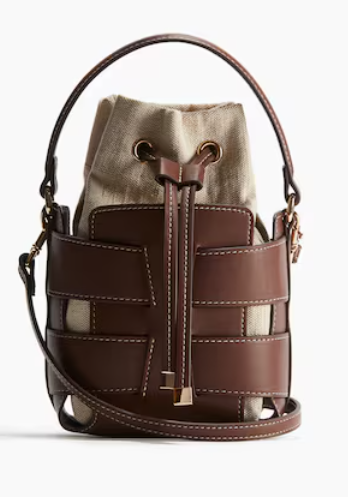
\includegraphics[width=2.5cm,clip,keepaspectratio]{1f8cefac125a428c8fb08ff110853ea3.png}
\end{textblock*}

% ---------- En-tête ---------------------------------------------
\begin{center}
  {\fontsize{44pt}{24pt}\selectfont\bfseries Judikael Mourouvin}

  \bigskip
  {\Large Technicien informatique \& marketing digital}

  \bigskip\bigskip
  \faMapMarker~Route de COCOYER\ 97190 GOSIER
  \quad\faEnvelope~\href{mailto:jkmou971@gmail.com}{jkmou971@gmail.com}

  \bigskip
  % Badge LinkedIn (retirez-le si inutile)
  \faPhone~ +590 0690 91 14 48
  \quad \faLinkedin\ \href{}{}
 

  \vspace{-0.3cm}
  \fullrule
\end{center}

% ---------- Profil ----------------------------------------------
\cvsection{Profil}
\hspace*{2cm}%
Passionné par l’informatique et le marketing digital, je possède une solide expérience en support technique, administration de systèmes et gestion de projets numériques. Mon année d’alternance à la DSI de la Mairie du Gosier m’a permis de développer des compétences pointues en analyse des besoins utilisateurs et en déploiement de solutions adaptées. Autonome et rigoureux, je suis capable d’assurer la maintenance d’un parc informatique tout en contribuant à la stratégie digitale d’une organisation. Je souhaite désormais mettre mon expertise au service de nouveaux projets, avec efficacité et sens du résultat.

\medskip\fullrule

% ---------- Expérience -----------------------------------------
\cvsection{Expérience}
\begin{adjustwidth}{2cm}{0pt}      % ← retrait gauche 1.3 cm
  
\colorbox{maincolor}{%
  \begin{minipage}{\linewidth}
    \textbf{Alternant en Marketing Digital} \\ Mairie du Gosier – DSI \\ 2023-2024
    \begin{itemize}
      \item Piloté des projets numériques municipaux et assuré leur mise en production dans les délais. \item Analysé les besoins des agents puis déployé des solutions adaptées, améliorant l’efficacité opérationnelle. \item Formé les utilisateurs et contribué au développement de la présence digitale de la collectivité.
    \end{itemize}
  \end{minipage}}

\vspace{3mm}


\colorbox{maincolor}{%
  \begin{minipage}{\linewidth}
    \textbf{Animateur de la zone informatique} \\ Pôle Emploi, Gosier \\ 2022-2023
    \begin{itemize}
      \item Assuré le support de premier niveau auprès des usagers, réduisant les temps d’attente et les incidents récurrents. \item Configuré et maintenu le parc informatique pour garantir une disponibilité continue des postes. \item Diagnostiqué et résolu les anomalies matérielles et logicielles, augmentant la satisfaction utilisateur.
    \end{itemize}
  \end{minipage}}

\vspace{3mm}


\colorbox{maincolor}{%
  \begin{minipage}{\linewidth}
    \textbf{Stagiaire Informaticien} \\ Numerika, Baie-Mahault \\ 2020-2021
    \begin{itemize}
      \item Installé et entretenu les équipements informatiques afin d’optimiser leurs performances. \item Assuré un support technique réactif aux collaborateurs, limitant les interruptions de service.
    \end{itemize}
  \end{minipage}}
\end{adjustwidth}

\medskip\fullrule

% ---------- Éducation ------------------------------------------
\cvsection{Éducation}
\begin{adjustwidth}{2cm}{0pt}      % ← même retrait
  
    \begin{tabularx}{\linewidth}{@{}c >{\RaggedRight\arraybackslash}X@{}}
    \textcolor{sidetext}{\faGraduationCap} &
    \textbf{Bachelor Marketing Digital} \\
    & CFA IUTS \\
    & \textit{2023-2024} \\
    \end{tabularx}
    \begin{itemize}[leftmargin=*]
  \item Stratégies de communication en ligne et gestion de contenu.
  \item Analyse de données marketing et optimisation de campagnes digitales.
\end{itemize}
\vspace{3mm}

    \begin{tabularx}{\linewidth}{@{}c >{\RaggedRight\arraybackslash}X@{}}
    \textcolor{sidetext}{\faGraduationCap} &
    \textbf{BTS Systèmes Numériques option Informatique et Réseaux} \\
    & Lycée de Chevalier Saint-Georges, Abymes \\
    & \textit{2019-2021} \\
    \end{tabularx}
    \begin{itemize}[leftmargin=*]
  \item Architecture des réseaux et administration de systèmes.
  \item Maintenance matérielle et logicielle, support technique aux utilisateurs.
\end{itemize}
\end{adjustwidth}

\medskip\fullrule

% ---------- Compétences -----------------------------------------
\cvsection{Compétences}

\hspace*{2cm}%
\begin{tabular}{@{}p{0.25\linewidth}p{0.18\linewidth}p{0.18\linewidth}p{0.18\linewidth}}\cicon Administration & \cicon Réseaux & \cicon Maintenance & \cicon Support \\
\cicon Marketing & \cicon Digital & \cicon Configuration & \cicon Diagnostic \\
\cicon Formation & \cicon Assistance & ~ & ~ \\\end{tabular}   % grille 3 lignes × 4 colonnes

\end{document}
